\chapter{\acrfull{iam}}


\section{Umfang}
In diesem Kaptiel werden die On-Premise \acrfull{iam} Lösungen erläutert.
Die Federation \acrshort{iam} haben einen sehr spezifischen Use-Cases und sind hauptsächlich bei Cloud-First Archtitekturen zu finden. Daher sind diese in diesem Dokument ausserhalb des Umfangs und werden nicht weiter behandelt.

\section{\acrshort{iam} Varianten}
Ein \acrfull{iam} ist ein zentrales System welches die Entitäten, wie Benutzeraccounts und Computer, erfassen kann. Zudem können Berechtigungen auf Entitäten in einer Domäne verwaltet.\\

\textbf{Braucht es ein IAM?}\\
Es ist grundsätzlich möglich ohne ein IAM System zu arbeiten, wobei der Aufwand für das Management der Userverwaltung auf allen Maschinen schnell den Rahmen des Budgets sprengt.
Der allgemeine Konsenus ist, dass ab 15 aktiven Bentuzern ein IAM verwendet werden soll.\\

Eine IAM Lösung bringt viele Vorteile, gleichzeitig birgt es auch Risiken.\\

\begin{minipage}{\linewidth}
    \begin{multicols}{2}
        \begin{table}[H]
            \begin{center}
                \textbf{Vorteile:}
                \begin{itemize}
                    \item zentrales Accountmanagement
                    \item zentrales Accessmanagement
                    \item schnelle Skalierung Server/Client Umgebung
                    \item single Source of Truth\footnote{\href{https://de.wikipedia.org/wiki/Single\_Point\_of\_Truth}{https://de.wikipedia.org/wiki/Single\_Point\_of\_Truth}}
                    \item Policysystem zur Konfiguration von Client
                    \item meist gebündelt mit nützlichen Features\footnote{\acrshort{dhcp}, \acrshort{dns}, \acrshort{ntp}, \acrshort{ca} etc. (Produktabhängig)}
                    \item Single Sign-On
                \end{itemize}
            \end{center}
            \caption{Vorteile IAM}
        \end{table}
        \begin{table}[H]
            \begin{center}
                \textbf{Nachteile:}
                \begin{itemize}
                    \item hoher initial Aufwand
                    \item höchste Priorität eines Angreifers
                    \item anfällig auf Misskonfigurationen
                    \item abhängigkeit eines stabilen Systems
                \end{itemize}
            \end{center}
            \caption{Nachteile IAM}
        \end{table}
    \end{multicols}
\end{minipage}

\vspace{1cm}
Wie bei vielem ist es wichtig das richtige Produkt für seine Umgebung zu finden. Als nächstes werden zwei, im Markt beliebte Produkte vorgestellt.

\subsection{Active Directory}
Active Directory ist ein Produkt von Microsoft und kann exklusiv auf einem Microsoft Windows Server installiert werden. Active Directory ist einfach zu installieren, wobei die Konfiguration Herausforderungen mit sich bringen kann.\\

Active Directory ist mit mehr als 80\% Marktanteil der Marktführer.
Das Produkt bietet alle grundlegenden Funktionen wie User-, Geräte- und Berechtigungsverwaltung.
Ausserdem lässt sich Active Directory integrieren mit anderen Windows Server Funktionen wie \acrshort{dhcp}, \acrshort{dns}, \acrshort{ntp} und weiteren externen Funktionen von anderen Anbietern.
Vorallem in Windowsnetzwerken ist die Integration sehr gut und intuitiv.\\


Active Directory bietet in fast allen Fällen was ein KMU braucht und viel mehr. Deshalb ist die Wahl von Active Directory für KMUs meist die richtige Wahl. Es gibt nur wenige sehr spezifische Fälle in denen ein anderes Produkt besseren Nutzen erbringt.


\subsection{FreeIPA}
FreeIPA ist eine Open-Source Implementation eines IAMs, entwickelt durch die Community und Upstream von Red Hat Identity Management. Exklusiv verfügbar auf RPM-basierten Linux Systemen.\\

FreeIPA bietet von den Features einen ähnlichen Umfang wie Active Directory, aber mit dem grossen Unterschied, dass die Hauptzielgruppe Linux Server und Clients sind. Es werden auch User-, Geräte- und Berechtigungsverwaltung, \acrshort{dhcp}, \acrshort{dns}, \acrshort{ntp} und viele weitere einfache, bis zu komplexen Funktionen angeboten.\\

FreeIPA ist eine gute Wahl in exklusiven Linuxnetzwerken. Für KMUs ist in den meisten Fällen FreeIPA die falsche Wahl und Active Directory sollte vorgezogen werden.


\section{Betreiben eines IAMs}
Das Betreiben eines IAMs kann Herausforderungen bieten.
Es gibt viele Dinge zu beachten.
Das wichtigste ist es ein Verständnis zu erlangen wie kritisch das IAM System ist.
Ein Ausfall des IAM Systems kann das ganze Netzwerk beeinträchtigen und bewirken, dass das Arbeiten für die ganze Firma schwerer, bis unmöglich wird.
Eine Misskonfiguration kann die Türe für einen Cybersecurityvorfall öffnen.
Das IAM ist oftmals das primäre Angriffsziel eines Angreifers, da ab diesem alle Systeme \& und deren Zugriff verwaltet wird.\\

Um die Angriffsfläche und somit das Risiko zu minimieren sollten die unten beschriebenen Konzepte beachtet und wenn möglich strikt implementiert werden.

\subsection{Least Privilege}
Das ``least privilege principle'' ist ein grundlegender Security Best Practice, denn man überall wieder findet.\\

Das Prinzip besagt jeder Benutzer soll genau soviel Rechte haben, wie er für seine tägliche Arbeit benötigt. Alles weitere soll blockiert werden.
Somit kann die Angriffsfläche bei Vorfällen massiv verringert werden.\\

Für privilegierte Benutzer wie z.B. ein Systemadministrator sollen zusätzliche, spezielle Accounts bereitgestellt werden.
Denn die meiste Arbeit kann mit einem nicht privilegierten Nutzer verrichtet werden.\\

Zusätzlich soll auch beachtet werden, dass es keine ``Masteraccounts'' gibt, welche alle Rechte besitzen.
Den diese sind für Angreifer besonders interessant und für das Unternehmen gefährlich.


\subsection{Persönliche Accounts}
Es muss versucht werden die Anzahl unpersönliche Accounts auf ein minimum beschränkt zu halten.
Bei einem Incident sind die Logs ausschlaggebend.\\

Arbeiten alle Benutzer mit dem Account ``Finanzen'' ist es schwer Rückschlüsse zu ziehen, wo kritische Aktionen oder ilegitime Zugriffe passiert sind.
In einem Vorfall wäre es klar, dass der Verstoss mit dem Account ``Finanzen'' passiert ist, aber welcher der 10 Personen die den Account benutzen den Verstoss begangen hat ist schwer, bis unmöglich Rückzuschliessen.

\subsection{Rollen als Berechtigungen}
Unternehmungen sind ermutigt Jobprofile zu erstellen, um geeignetes Personal zu finden.
Es ist ähnlich in der Verteilung von Benutzerrechten.
Eine Person ist angestellt um eine bestimmte Arbeit zu verrichten.
Diese Zuteilung wird nun auf eine Rolle abgebildet.
Die Rolle mit den Rechten erhalten alle Angestellten mit dem gleichen Auftrag.
Oftmals werden Rollen in einem IAM ``Gruppen'' genannt, welcher man Benutzer und andere Gruppen hinzufügen kann.\\

Das Verteilen von Rollen erleichtert den Überblick der einzelnen Berechtigungen in der Unternehmung.
Bei individual Berechtigungen verliert man schnell den Überblick.
Mit administrativen Wechseln wie interne Umorientierungen kann es dazu führen, dass Nutzer zu viele Berechtigungen für Ihren Job haben und somit das ``least privilege principle'' verletzen.
Mit Rollen kann bei internen Wechseln lediglich die alte Rolle entfernt und die neue Rolle hinzugefügt werden.


\subsection{Automatische Benutzerverwaltung}
Es ist empfohlen die Benutzerverwaltung zu automatisieren oder einen klaren Prozess festzulegen.
Dies betrifft vorallem die Benutzer, welche das Unternehmen verlassen.
Die Accounts sollten beim Austritt deaktiviert und nach einer definierten Zeit gelöscht werden.


\subsection{Zuständigkeitsbereich eines IAM}
Es kann eine Herausforderung entstehen, wenn man alle seine Geräte an das IAM anbinden will.\\

Im Idealfall sind alle Geräte an das IAM angebunden.
Es gibt aber auch Instanzen, in welchen diese Lösung nicht wirtschaftlich vertretbar ist.
Das geht in Ordnung.
Bei solchen Geräten sollte sich überlegt werden, wie sie adäquat geschützt werden können.

\subsection{IAM Schlusswort}
Ein IAM kann Agilität, Komfort und Sicherheit bringen.
Mit den Vorteilen bringt ein IAM auch Risiken, wie Sicherheitsbedenken und Abhängigkeit für den produktiven Betrieb.
Daher sollte ein IAM bestmöglich geschützt werden.
Editorberechtigung im IAM sollten nur Personen zustehen, welche diese auch wirklich brauchen (least privilege).

In den meisten Fällen ist ein IAM die beste Lösung.
Der grösste Teil der Vorfälle kann mit den zuvor genannten Konzepten mitigiert oder sogar ganz vermieden werden.


\section{Active Directory Best Practices}
\subsection{Passwortrichtlinien}
Es gibt verschiedene Möglichkeiten, wie Angreifer an Passwörter kommen können.
Darunter gehören zum Beispiel:
\begin{itemize}
    \item Bruteforce Attacken: Auf einem Account verschiedene Passwörter testen.
    \item Spraying Attacken: Ein Passwort mit verschiedenen Accounts testen.
    \item Dictionary Attacks: Bruteforce-Attacke mit einer Liste von bekannten Passwörtern.
    \item Social-Engineering: Angreifer versuchen das Passwort direkt vom Benutzer zu bekommen.
\end{itemize}

Best Practice für die Passwortvorgaben für User und Administratoren sind folgend\footnote{Zugriff: 16.04.2022 \cite{nist-digital-identity-guidelines}}:
\begin{itemize}
    \item Lange Passwörter sind besser als komplexe Passwörter.
    \item Lange Passwörter müssen \textbf{nicht} in einem gewissen Interval gewechselt werden.
    \item Passwort Hinweise beim Login sollten deaktiviert werden. (Standard in AD)
    \item Anzahl möglicher Anmeldeversuche sollte eingeschränkt werden.
\end{itemize}

\acrshort{nist} empfiehlt für die mindestlänge eines Passwortes 8 Zeichen.
Dieser Guide empfiehlt jedoch mindestens 12 Zeichen.
Hier ein Vergleich von einem 8-Stelligen und einem 12-Stelligen Passwort, welches Gross- und Kleinschreibung und Zahlen enthält\footnote{Berechnet mit: https://www.passwortcheck.ch/}:\\
\begin{minipage}{0.5\linewidth}
    \begin{figure}[H]
        \centering
        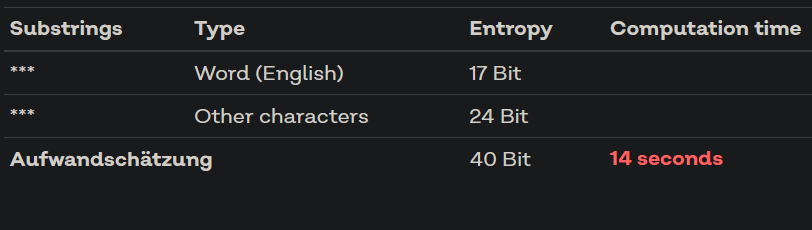
\includegraphics[width=\linewidth]{../img/IAM/8-characters.png}
        \caption{Passwort mit 8 Stellen}
    \end{figure}
\end{minipage}
\begin{minipage}{0.5\linewidth}
    \begin{figure}[H]
        \centering
        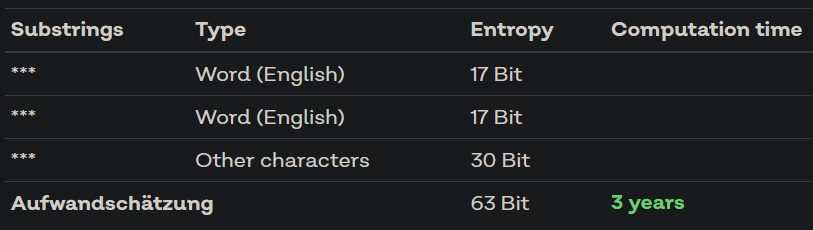
\includegraphics[width=\linewidth]{../img/IAM/12-characters.png}
        \caption{Passwort mit 12 Stellen}
    \end{figure}
\end{minipage}
\subsubsection{Group Policy für Passwortrichtlinien}
Die Passwortrichtlinien können per Group Policy gesetzt werden.
Im Group Policy Management existiert unter \textbf{Forest: <Domänen-Namen> $\rightarrow$ Domains $\rightarrow$ <Domänen-Namen>} die ``Default Domain Policy''.
In dieser setzt man unter \textbf{Computer Configuration $\rightarrow$ Policies $\rightarrow$ Windows Settings $\rightarrow$ Security Settings $\rightarrow$ Account Policies} folgende Richtlinien:\\

\begin{minipage}{0.5\linewidth}
    \textbf{Password Policy:}
    \begin{figure}[H]
        \centering
        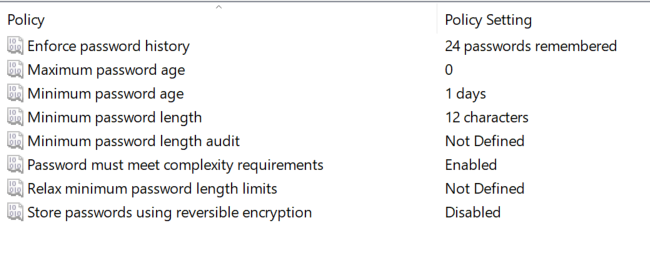
\includegraphics[width=\linewidth]{../img/IAM/default-password-policy.png}
        \caption{Passwortrichtlinien}
    \end{figure}
\end{minipage}
\begin{minipage}{0.5\linewidth}
    \textbf{Account Lockout Policy:}
    \begin{figure}[H]
        \centering
        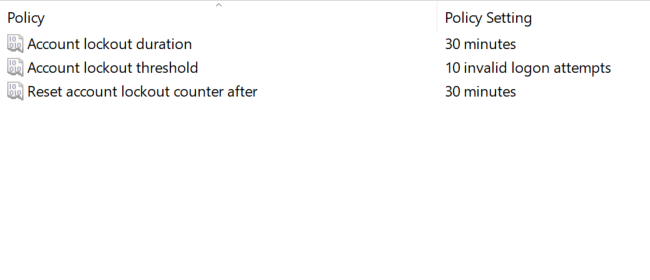
\includegraphics[width=\linewidth]{../img/IAM/account-lockout-policy.png}
        \caption{Account Lockout Richtlinien}
    \end{figure}
\end{minipage}\\

Die Group Policy kann nun so geschlossen werden.
In den AD Objekten der Benutzer ist nun unter ``Account'' ein Hacken bei ``Password never expires''.
Falls die Passwordrichtline vorher bei weniger als 12 Zeichen war, müssen nun die Benutzer noch aufgefordert werden, ihr Passwort zu ändern.
Dies kann mit Powershell gemacht werden:
\begin{lstlisting}
    Get-ADUser -SearchBase "<OU der Benutzer>" -Filter * | Set-ADUser -ChangePasswordAtLogon $True

    #Beispiel:
    Get-ADUser -SearchBase "OU=Employees,OU=Users,OU=Lab,DC=ba,DC=lab" -Filter * | Set-ADUser -ChangePasswordAtLogon $True
\end{lstlisting}

Dies sollte mit dem Management abgeklärt werden und die Benutzer sollten frühzeitig informiert werden.
Man kann auch zuerst die Mindestlänge in der Group Policy setzen und erst nach einem Zyklus, wenn alle Mitarbeitenden ihr Passwort auf die neue Länge gesetzt haben, die Option ``Maximum password age'' auf 0 setzen. \\

Bei der Passwortrichtlinie für Administratoren wird empfohlen, dass diese ihr Passwort weiterhin mindestens alle 180 Tage wechseln müssen.
Dazu kann eine neue Group Policy auf Höhe der \acrshort{ou} mit den Administratoren erstellt werden:
\begin{figure}[H]
    \centering
    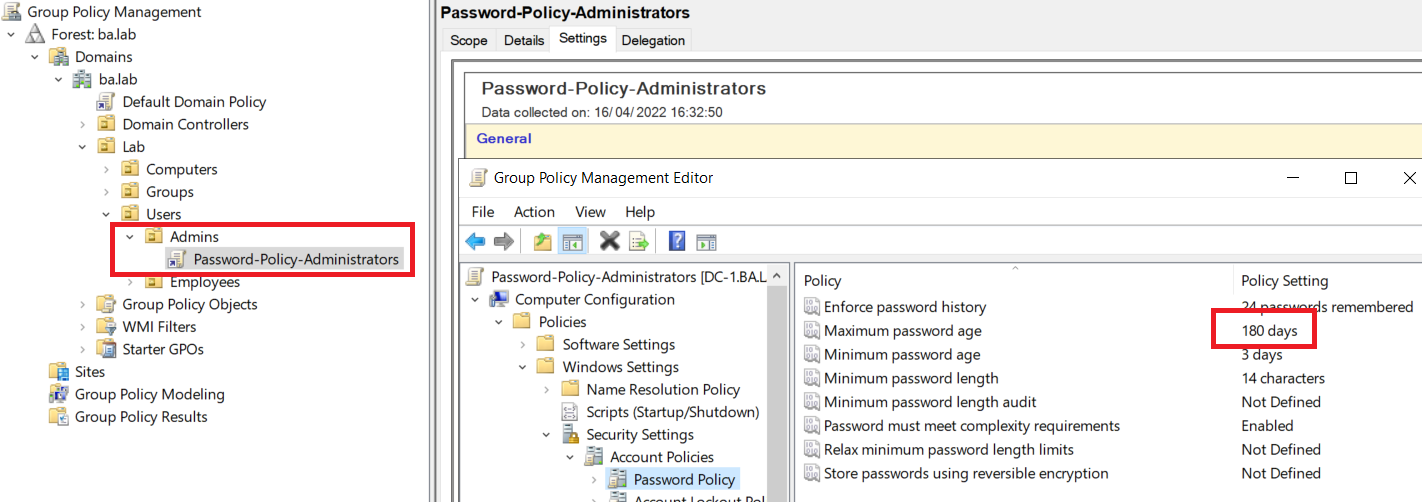
\includegraphics[width=0.7\linewidth]{../img/IAM/admin-password-policy.png}
    \caption{Passwortrichtlinien Administratoren}
\end{figure}
Die Account Lockout Policy bleibt gleich.

\subsection{Active Directory Auditing}
Active Directory bietet die Möglichkeit, Änderungen an Gruppen und Benutzern im Event Log festzuhalten.
Dies ist nützlich um nachvollziehen zu können, wann welche Änderungen gemacht wurden und zusammen mit Wazuh erkennen zu können, ob Änderungen gemacht wurden die nicht von Administratoren kamen.\\

Diese Logs müssen mit einer Group Policy aktiviert werden.
Im Group Policy Management existiert unter \textbf{Forest: <Domänen-Namen> $\rightarrow$ Domains $\rightarrow$ <Domänen-Namen> $\rightarrow$ Domain Controllers} die ``Default Domain Controllers Policy''.
In dieser setzt man unter \textbf{Computer Configuration $\rightarrow$ Policies $\rightarrow$ Windows Settings $\rightarrow$ Security Settings $\rightarrow$ Local Policies $\rightarrow$ Audit Policy} in der Richtlinie ``Audit account Management'' folgende Einstellungen:\\
\begin{figure}[H]
    \centering
    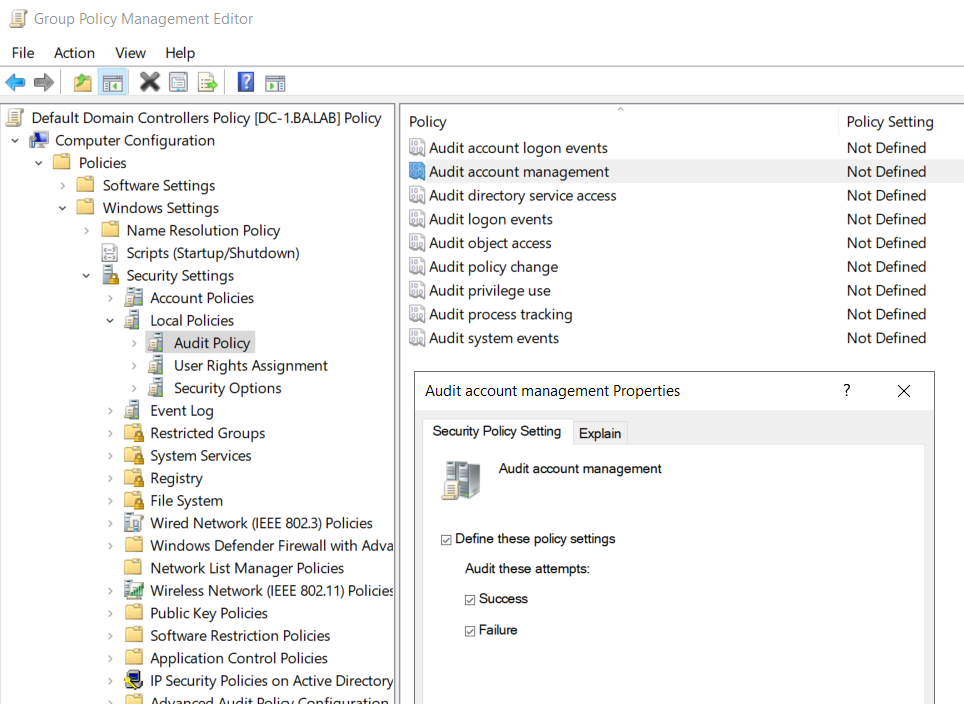
\includegraphics[width=0.7\linewidth]{../img/IAM/ad-account-management.png}
    \caption{Active Directory Audit Policy}
\end{figure}

\section{Intergration in Wazuh}
\subsection{Account Lockout}
Wenn ein Benutzer sein Passwort zu oft falsch eingibt (wenn aktiviert in der Group Policy), generiert Wazuh ein Alert.
Dieser sieht folgendermassen aus:
\begin{figure}[H]
    \centering
    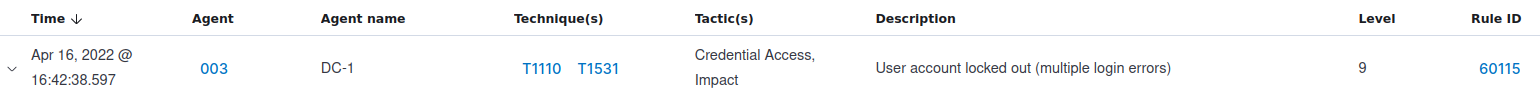
\includegraphics[width=\linewidth]{../img/IAM/account-lockout.png}
    \caption{Account Lockout Alert Beispiel}
\end{figure}

\subsection{Änderungen in AD}
Wazuh loggt standardmässig alle Änderungen in Active Directory.
Dies beihnaltet Änderungen an Accounts und Gruppen:
\begin{lstlisting}
    Security Enabled (Local|Global|Universal) Group (Created|Changed|Deleted)
    Security Enabled (Local|Global|Universal) Group Member (Added|Removed)
\end{lstlisting}
\begin{figure}[H]
    \centering
    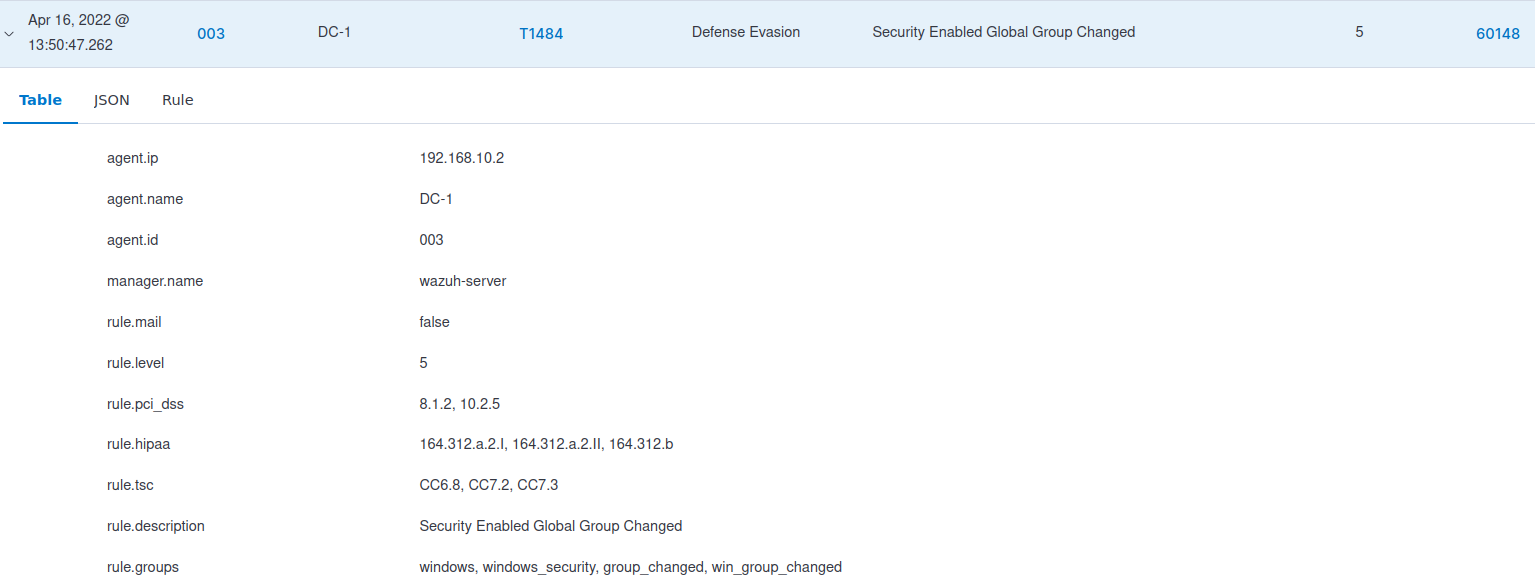
\includegraphics[width=0.7\linewidth]{../img/IAM/security-group-alert-example.png}
    \caption{Security Group Alert Beispiel}
\end{figure}

Zusätzlich gibt es noch Alert mit Level 12, falls eine Standardgruppe mit erhöhten Berechtigungen geändert wird.
Dazu gehören folgende Gruppen:
\begin{figure}[H]
    \centering
    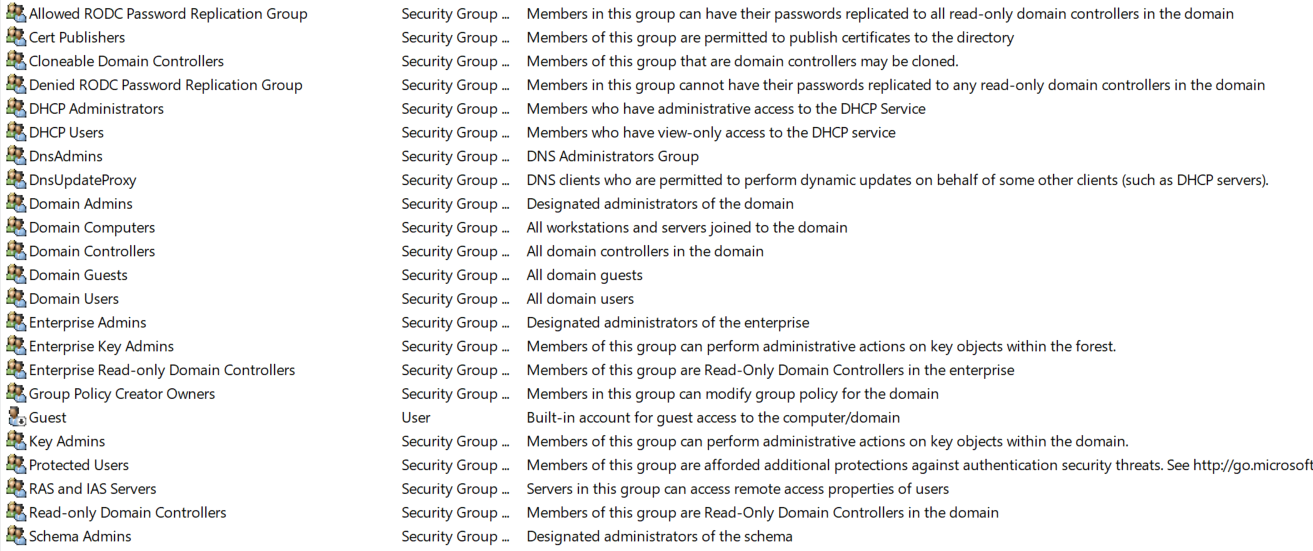
\includegraphics[width=0.7\linewidth]{../img/IAM/high-privilege-groups.png}
    \caption{Gruppen mit erhöhten Berechtigungen}
\end{figure}
Die Alerts sehen wie folgt aus:
\begin{figure}[H]
    \centering
    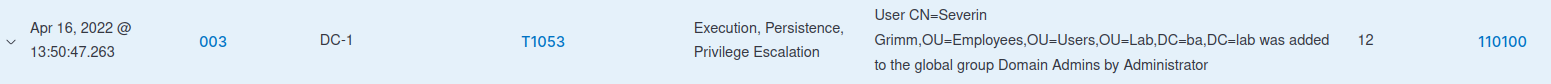
\includegraphics[width=\linewidth]{../img/IAM/alert-added-to-privilege-group.png}
    \caption{Security Group Level 12 Alert Beispiel}
\end{figure}